\documentclass[11pt,a4paper]{article}

% Image mode: pdf.
% Image paths stay relative. In PDF mode, place same-basename PDF conversions
% of the chapter SVG files in the assets/ directory beside this source.

\usepackage{iftex}
\ifPDFTeX
  \PackageError{handout}{This template requires XeTeX or Tectonic}{Compile with xelatex or tectonic.}
\fi

\usepackage[a4paper,top=18mm,bottom=20mm,left=20mm,right=20mm,headsep=6mm]{geometry}
\usepackage{fontspec}
\usepackage{xeCJK}
\usepackage{amsmath}
\usepackage{unicode-math}

% Font settings are intentionally visible in the generated .tex file.
% These defaults target the macOS machine used for the released PDF.
% Change the family names when compiling on another system.
\setmainfont{Songti TC}
\setsansfont{Heiti TC}
\setmonofont{Menlo}
\setCJKmainfont{Songti TC}
\setCJKsansfont{Heiti TC}
\setCJKmonofont{Heiti TC}
\setmathfont{STIX Two Math}
\XeTeXlinebreaklocale "zh"
\XeTeXlinebreakskip=0pt plus 1pt

\usepackage{xcolor}
\definecolor{HandoutBlue}{HTML}{215A91}
\definecolor{HandoutBlueLight}{HTML}{EEF5FC}
\definecolor{HandoutGreen}{HTML}{39715A}
\definecolor{HandoutGreenLight}{HTML}{EFF8F3}
\definecolor{HandoutGold}{HTML}{8A641C}
\definecolor{HandoutGoldLight}{HTML}{FFF8E8}
\definecolor{HandoutInk}{HTML}{253142}
\definecolor{HandoutMuted}{HTML}{667085}

\usepackage{graphicx}
\makeatletter
% Pandoc 3 emits an accessibility `alt` key for raster/PDF images. Older
% graphicx releases do not know that key, so accept it without changing layout.
\@ifundefined{KV@Gin@alt}{\define@key{Gin}{alt}{}}{}
\newsavebox\pandoc@box
\newcommand*\pandocbounded[1]{%
  \sbox\pandoc@box{#1}%
  \Gscale@div\@tempa{\textheight}{\dimexpr\ht\pandoc@box+\dp\pandoc@box\relax}%
  \Gscale@div\@tempb{\linewidth}{\wd\pandoc@box}%
  \ifdim\@tempb\p@<\@tempa\p@\let\@tempa\@tempb\fi
  \ifdim\@tempa\p@<\p@\scalebox{\@tempa}{\usebox\pandoc@box}%
  \else\usebox{\pandoc@box}%
  \fi
}
\makeatother
\usepackage{float}
\floatplacement{figure}{H}
% Pandoc uses LTcaptype=none for uncaptioned longtables. The caption package
% expects that name to exist as a counter even though it is never displayed.
\newcounter{none}
\usepackage{caption}
\captionsetup[figure]{labelformat=empty,labelsep=none,font=small}

\usepackage{booktabs,longtable,array,calc}
\usepackage{etoolbox}
\makeatletter
\patchcmd\longtable{\par}{\if@noskipsec\mbox{}\fi\par}{}{}
\makeatother

\usepackage[most]{tcolorbox}
\tcbuselibrary{breakable,skins}
\newtcolorbox{HandoutLearningMap}{
  enhanced,breakable,colback=HandoutBlueLight,colframe=HandoutBlue,
  boxrule=0.8pt,arc=1.5mm,left=3mm,right=3mm,top=2mm,bottom=2mm,
  before skip=8pt,after skip=10pt
}
\newtcolorbox{HandoutWorkedExample}{
  enhanced,breakable,colback=HandoutGreenLight,colframe=HandoutGreen,
  boxrule=0.65pt,arc=1.5mm,left=3mm,right=3mm,top=2mm,bottom=2mm,
  before skip=8pt,after skip=10pt
}
\newtcolorbox{HandoutSelfCheck}{
  enhanced,breakable,colback=HandoutGoldLight,colframe=HandoutGold,
  boxrule=0.65pt,arc=1.5mm,left=3mm,right=3mm,top=2mm,bottom=2mm,
  before skip=8pt,after skip=10pt
}

\usepackage{titlesec}
\titleformat{\section}{\sffamily\bfseries\Large\color{HandoutBlue}}{}{0pt}{}
\titleformat{\subsection}{\sffamily\bfseries\large\color{HandoutInk}}{}{0pt}{}
\titleformat{\subsubsection}{\sffamily\bfseries\normalsize\color{HandoutInk}}{}{0pt}{}
\titlespacing*{\section}{0pt}{1.4em}{0.55em}
\titlespacing*{\subsection}{0pt}{1.15em}{0.45em}
\titlespacing*{\subsubsection}{0pt}{0.9em}{0.35em}
\setcounter{secnumdepth}{-\maxdimen}

\usepackage{hyperref}
\usepackage{bookmark}
\IfFileExists{xurl.sty}{\usepackage{xurl}}{}
\urlstyle{same}
\hypersetup{
  colorlinks=true,
  linkcolor=HandoutBlue,
  urlcolor=HandoutBlue,
  citecolor=HandoutBlue,
  pdftitle={選物I-1 測量與不確定度},
  pdfsubject={物理},
  pdfcreator={Pandoc with the HighSchooContent LaTeX template}
}

\setlength{\parindent}{0pt}
\setlength{\parskip}{0.55em plus 0.15em minus 0.1em}
\setlength{\emergencystretch}{3em}
\setlength{\LTpre}{0.5em}
\setlength{\LTpost}{0.5em}
\renewcommand{\arraystretch}{1.18}
\providecommand{\tightlist}{%
  \setlength{\itemsep}{0pt}\setlength{\parskip}{0pt}}
\pagestyle{plain}


\begin{document}

\begin{tcolorbox}[
  enhanced,colback=white,colframe=HandoutBlue,boxrule=1.1pt,arc=2mm,
  borderline west={3pt}{0pt}{HandoutBlue},left=5mm,right=4mm,top=4mm,bottom=4mm
]
{\sffamily\small\bfseries\color{HandoutBlue}學生講義}\par
{\sffamily\bfseries\LARGE\color{HandoutInk}選物I-1 測量與不確定度}\par
\vspace{0.35em}{\large 測量結果由估計值與不確定度共同構成}\par
\vspace{0.45em}{\small\color{HandoutMuted}%
科目：物理
\quad 課程：普通高中選修物理 I
\quad 版本：學生版｜核心＋理解
\quad 校訂：2026-08-25
}\par
\vspace{0.25em}{\small\color{HandoutMuted}範圍：現行選修主線}\par
\end{tcolorbox}


\begin{HandoutLearningMap}

\subsection{本章核心關係}\label{ux672cux7ae0ux6838ux5fc3ux95dcux4fc2}

\begin{enumerate}
\def\labelenumi{\arabic{enumi}.}
\tightlist
\item
  \textbf{測量結果包含哪些資訊？}──同一個量反覆測量，結果通常不完全相同，因此須同時報告估計值與不確定度。
\item
  \textbf{不確定度從哪裡來？}──被測物、儀器、測量者與環境都可能貢獻。
\item
  \textbf{怎麼把反覆測量與儀器解析度合成一個不確定度？}──分別作 A 類、B 類評估，再用平方和開根號合成。
\item
  \textbf{帶有不確定度的量相加、相減、相乘或相除時，結果怎麼報告？}──獨立測量的貢獻仍以平方和開根號組合。
\item
  \textbf{因次分析能檢查什麼？}──等式兩邊與可相加各項的因次必須一致。
\end{enumerate}

{藍色：現行核心}
{青綠：理解支援}
{紫色：超出本章必學邊界}

111--115 官方題本固定窗口中，3/5 份分科物理直接使用測量與不確定度方法；3/5 份學測自然直接檢核單位或因次基礎。完整 GUM 計算不屬於學測固定範圍，這組統計也不預測下一屆考題。

\end{HandoutLearningMap}

\section{1. 測量結果包含估計值與不確定度}\label{ux6e2cux91cfux7d50ux679cux5305ux542bux4f30ux8a08ux503cux8207ux4e0dux78baux5b9aux5ea6}

用同一把尺反覆量同一張桌子，讀數可能出現些微差異。這不一定代表有人粗心；桌緣不完全筆直、刻度有限、視線角度與室溫變化，都會影響結果。

現代測量採用\textbf{不確定度（uncertainty）}描述：根據現有資料與方法，我們對待測量知道到什麼程度。記號先約定如下：

\begin{itemize}
\tightlist
\item
  \(x\)：待測的物理量。
\item
  \(X\)：由資料得到的最佳估計值。
\item
  \(u\)：標準不確定度，必為非負數，與 \(X\) 有相同單位。
\end{itemize}

測量結果寫成

\[
\boxed{x=X\pm u}.
\]

本章依 114 教材，把「最佳估計值與標準不確定度」簡記為 \(x=X\pm u\)。若根據量測模型，可合理歸因於待測量的可能值近似呈常態分布，且 \(u\) 可視為該分布的標準差，則 \(X-u\) 到 \(X+u\) 約涵蓋 \(68.3\%\) 的可能值。這是特定假設下的解讀，不是所有 \(X\pm u\) 都自動具有 \(68.3\%\) 涵蓋率，也不保證真值必在其中。

\subsection{不確定度的四個來源}\label{ux4e0dux78baux5b9aux5ea6ux7684ux56dbux500bux4f86ux6e90}

{\def\LTcaptype{none} % do not increment counter
\begin{longtable}[]{@{}
  >{\raggedright\arraybackslash}p{(\linewidth - 4\tabcolsep) * \real{0.3333}}
  >{\raggedright\arraybackslash}p{(\linewidth - 4\tabcolsep) * \real{0.3333}}
  >{\raggedright\arraybackslash}p{(\linewidth - 4\tabcolsep) * \real{0.3333}}@{}}
\toprule\noalign{}
\begin{minipage}[b]{\linewidth}\raggedright
來源
\end{minipage} & \begin{minipage}[b]{\linewidth}\raggedright
要問的問題
\end{minipage} & \begin{minipage}[b]{\linewidth}\raggedright
例子
\end{minipage} \\
\midrule\noalign{}
\endhead
\bottomrule\noalign{}
\endlastfoot
被測物 & 要測的量本身是否清楚、穩定？ & 桌緣粗糙、液面晃動、物體受熱膨脹 \\
儀器 & 儀器能分辨到多細？是否已校準？ & 尺的刻度有限、碼錶走時偏差 \\
測量者 & 判讀與操作是否會改變結果？ & 視差、按碼錶的反應時間 \\
環境 & 外界條件是否在測量時改變？ & 溫度、氣流、振動、電源波動 \\
\end{longtable}
}

\begin{HandoutWorkedExample}

\subsection{完整示範｜不確定度決定兩個結果能否分辨}\label{ux5b8cux6574ux793aux7bc4ux4e0dux78baux5b9aux5ea6ux6c7aux5b9aux5169ux500bux7d50ux679cux80fdux5426ux5206ux8fa8}

同一零件以兩套方法量得直徑

\[
d_A=(10.02\pm0.05)\ \mathrm{mm},\qquad
d_B=(10.11\pm0.04)\ \mathrm{mm}.
\]

若兩套方法的不確定度可視為獨立，直接比較差值

\[
D=d_B-d_A=0.09\ \mathrm{mm}.
\]

差值的合成標準不確定度為

\[
u_D=\sqrt{(0.05)^2+(0.04)^2}=0.064\ \mathrm{mm}.
\]

因此標準不確定度層級可寫成

\[
D=(0.090\pm0.064)\ \mathrm{mm}.
\]

比較兩個結果是否已清楚分開，須先指定涵蓋標準。若採常用的涵蓋因子 \(k=2\)，擴展不確定度

\[
U_D=ku_D=2(0.064)=0.128\ \mathrm{mm}\approx0.13\ \mathrm{mm}.
\]

差值的約 \(k=2\) 涵蓋區間為 \(0.09\pm0.13\ \mathrm{mm}\)，包含 0；現有證據尚未把兩方法的結果清楚區分。兩個 \(X\pm u\) 區間是否重疊可提供直觀，但 \(\pm1u\) 不是通用的判定門檻。正式比較應對差值 \(D\) 合成 \(u_D\)，再依任務指定的涵蓋因子或決策規則判讀。

\end{HandoutWorkedExample}

\begin{HandoutWorkedExample}

\subsection{完整示範｜由標準不確定度作門檻判讀}\label{ux5b8cux6574ux793aux7bc4ux7531ux6a19ux6e96ux4e0dux78baux5b9aux5ea6ux4f5cux9580ux6abbux5224ux8b80}

某電流感測器在指定工作狀態下的量測結果為

\[
I=(12.46\pm0.08)\ \mathrm{mA}.
\]

其中 \(12.46\ \mathrm{mA}\) 是最佳估計值，\(0.08\ \mathrm{mA}\) 是標準不確定度。校準資料支持近似常態分布；設備的保護規則採涵蓋因子 \(k=2\)，並以量測區間上界是否低於 \(12.80\ \mathrm{mA}\) 作判定。

\textbf{步驟 1──求擴展不確定度}

\[
U=k u=2(0.08\ \mathrm{mA})=0.16\ \mathrm{mA}.
\]

\textbf{步驟 2──寫出 \(k=2\) 量測區間}

\[
12.46-0.16\le I\le12.46+0.16,
\]

即

\[
12.30\ \mathrm{mA}\le I\le12.62\ \mathrm{mA}.
\]

\textbf{步驟 3──依指定規則判讀}

量測區間上界為 \(12.62\ \mathrm{mA}\)，低於保護門檻 \(12.80\ \mathrm{mA}\)；依這項 \(k=2\) 判定規則，現有量測支持設備在門檻內運作。這個結論同時使用最佳估計值、不確定度、涵蓋因子與事先指定的決策門檻。

\end{HandoutWorkedExample}

\subsection{真值未知時，以不確定度評估測量品質}\label{ux771fux503cux672aux77e5ux6642ux4ee5ux4e0dux78baux5b9aux5ea6ux8a55ux4f30ux6e2cux91cfux54c1ux8cea}

真值通常無法直接知道，因此誤差也無法直接算出。國際通用的 GUM 架構改以「可由資料與儀器評估的不確定度」報告測量品質，回答現有證據能支持多精細的結論。

\subsection{不確定度支撐工程、醫療與導航決策}\label{ux4e0dux78baux5b9aux5ea6ux652fux6490ux5de5ux7a0bux91abux7642ux8207ux5c0eux822aux6c7aux7b56}

讀數連同不確定度，才能判斷證據是否足以支撐決策。零件尺寸靠近公差邊界時，量測不確定度會影響「放行」或「重工」的風險，因此設備須校準，判定規則也須預先訂定。醫療檢測接近處置門檻時，判讀須結合方法不確定度、重測與臨床資訊。

衛星定位先量訊號傳播時間，再乘光速換成距離；時間誤差因此會轉成距離誤差。光在 \(1\ \mathrm{ns}\) 內約走 \(0.30\ \mathrm m\)，所以衛星鐘、接收器鐘、電離層模型與軌道資料都必須校正。定位系統從多筆帶不確定度的距離資料估計最合理的位置，並報告可信程度。

\begin{HandoutSelfCheck}

\subsection{練習}\label{ux7df4ux7fd2}

\begin{enumerate}
\def\labelenumi{\arabic{enumi}.}
\tightlist
\item
  量水溫時，溫度計最小刻度有限，而且水仍在緩慢降溫。這兩項分別屬於哪個來源？
\item
  長度報告為 \((25.4\pm0.2)\ \mathrm{cm}\)。寫出最佳估計值、不確定度與兩者單位。
\item
  甲結果為 \((8.00\pm0.03)\ \mathrm{s}\)，乙結果為 \((8.00\pm0.20)\ \mathrm{s}\)。哪一個結果提供較細的分辨能力？
\item
  校準證書指出秤的讀值可能共同偏高。這項資訊由「多量幾次」取得，還是由重複數據以外的資料取得？
\end{enumerate}

\textbf{答案：}1. 刻度有限屬於儀器；水溫隨時間改變屬於被測物在指定條件下不穩定。2. \(X=25.4\ \mathrm{cm}\)、\(u=0.2\ \mathrm{cm}\)。3. 甲；兩者中心相同，甲的 \(u\) 較小。4. 校準證書屬於重複數據以外的資訊，後續以 B 類方式評估。

\end{HandoutSelfCheck}

\section{2. 理解支援｜準確與精密描述不同品質}\label{ux7406ux89e3ux652fux63f4ux6e96ux78baux8207ux7cbeux5bc6ux63cfux8ff0ux4e0dux540cux54c1ux8cea}

{C2 理解支援｜最低版本可略}

反覆測量的結果很集中，稱為\textbf{精密（precise）}；測量結果接近可接受的參考值，稱為\textbf{準確（accurate）}。兩者回答不同問題：

{\def\LTcaptype{none} % do not increment counter
\begin{longtable}[]{@{}llr@{}}
\toprule\noalign{}
判讀 & 看什麼 & 只靠反覆測量能否判定？ \\
\midrule\noalign{}
\endhead
\bottomrule\noalign{}
\endlastfoot
精密度 & 多次讀數彼此是否集中 & 可以由散布程度判斷 \\
準確度 & 結果是否接近可信參考值 & 不一定；需要參考值或校準資訊 \\
\end{longtable}
}

一把沒有歸零的秤可能每次都讀得非常接近，卻整批偏高：它很精密，但不準確。反過來，數據散得很開，即使平均值碰巧接近參考值，也不能說每次測量都很精密。

\subsection{常見錯誤｜多量幾次能解決所有問題}\label{ux5e38ux898bux932fux8aa4ux591aux91cfux5e7eux6b21ux80fdux89e3ux6c7aux6240ux6709ux554fux984c}

增加測量次數可以降低由隨機散布造成的 A 類不確定度，卻不會自動修正共同偏移。例如秤固定多讀 \(5\ \mathrm{g}\)，量一百次的平均仍會多讀約 \(5\ \mathrm{g}\)；應先校準或改進方法。

\begin{HandoutSelfCheck}

\subsection{練習}\label{ux7df4ux7fd2-1}

甲組讀數為 \(10.1,10.1,10.1,10.1\)，可信參考值是 \(10.5\)；乙組讀數為 \(10.3,10.5,10.7,10.5\)。哪一組較精密？能否只看甲組的集中程度就說它較準確？

\textbf{答案：}甲組較精密，但整批離參考值較遠；不能因讀數集中就宣稱較準確。

\end{HandoutSelfCheck}

\section{3. A 類與 B 類依資訊來源分類}\label{a-ux985eux8207-b-ux985eux4f9dux8cc7ux8a0aux4f86ux6e90ux5206ux985e}

\subsection{A 類評估：由重複測量的統計散布得到}\label{a-ux985eux8a55ux4f30ux7531ux91cdux8907ux6e2cux91cfux7684ux7d71ux8a08ux6563ux5e03ux5f97ux5230}

在相同測量條件下，對同一物理量作 \(N\ge2\) 次彼此獨立的重複測量，得到 \(x_1,x_2,\ldots,x_N\)。先算平均值：

\[
\bar x=\frac{1}{N}\sum_{i=1}^{N}x_i.
\]

再以\textbf{樣本標準差}描述單次讀數的散布：

\[
s=\sqrt{\frac{1}{N-1}\sum_{i=1}^{N}(x_i-\bar x)^2}.
\]

因為平均值 \(\bar x\) 已由這 \(N\) 筆資料算出，所有偏差的和必為 \(0\)，只有 \(N-1\) 個偏差能自由改變，所以分母使用 \(N-1\)。若資料有明顯漂移或測量條件持續改變，不能直接套用 \(u_A=s/\sqrt N\)。

我們關心的是平均值有多穩定，因此 A 類標準不確定度為

\[
\boxed{u_A=\frac{s}{\sqrt N}}.
\]

\(s\) 描述單次讀數通常散多開；\(u_A\) 描述由 \(N\) 次資料所得平均值的不確定程度。兩者不能混用。

\begin{figure}
\centering
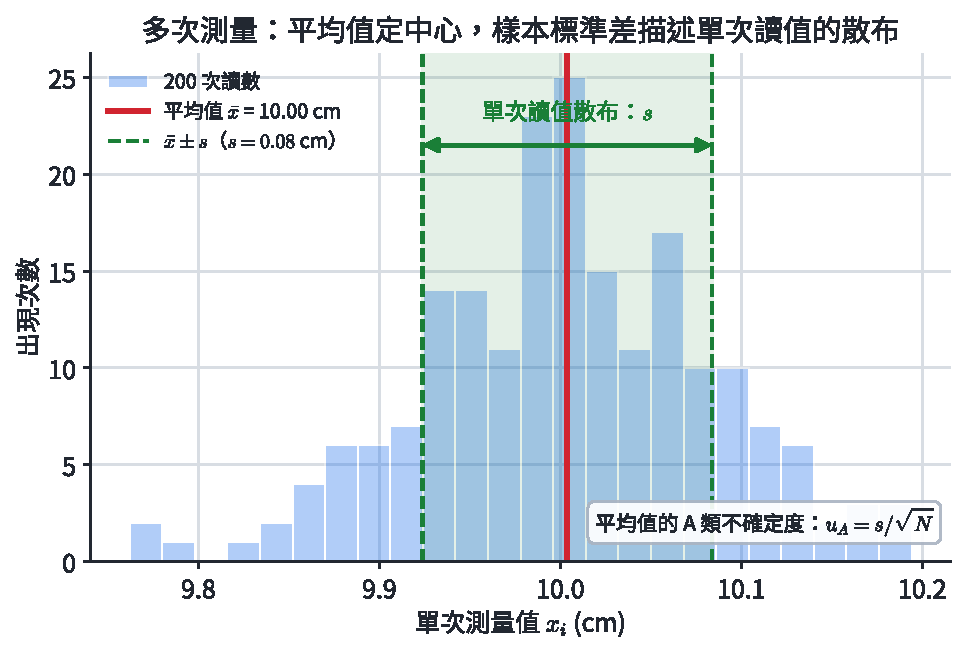
\includegraphics[width=0.96\linewidth,height=\textheight,keepaspectratio,alt={圖 1｜同一組重複讀數中，樣本標準差 s 描述單次讀數的散布；u\_A=s/\textbackslash sqrt N 描述平均值的不確定程度。}]{assets/選物I-1-多次測量分布.pdf}
\caption{圖 1｜同一組重複讀數中，樣本標準差 \(s\) 描述單次讀數的散布；\(u_A=s/\sqrt N\) 描述平均值的不確定程度。}
\end{figure}

\subsection{B 類評估：由儀器、資料或其他非重複統計資訊得到}\label{b-ux985eux8a55ux4f30ux7531ux5100ux5668ux8cc7ux6599ux6216ux5176ux4ed6ux975eux91cdux8907ux7d71ux8a08ux8cc7ux8a0aux5f97ux5230}

B 類評估由這組重複數據以外的資訊取得，例如：

\begin{itemize}
\tightlist
\item
  引用手冊、文獻或校正證書所給的不確定度時，依其說明採用。
\item
  直接由有刻度的儀器讀值，若把解析度造成的可能讀值建模為「以顯示值為中心、寬度為一個最小刻度 \(d\) 的均勻分布」，則
\end{itemize}

\[
\boxed{u_B=\frac{d}{2\sqrt3}}.
\]

這裡不是把最小刻度直接除以 2。\(d/2\) 是均勻分布區間的半寬；換成標準不確定度還要再除以 \(\sqrt3\)。

\begin{figure}
\centering
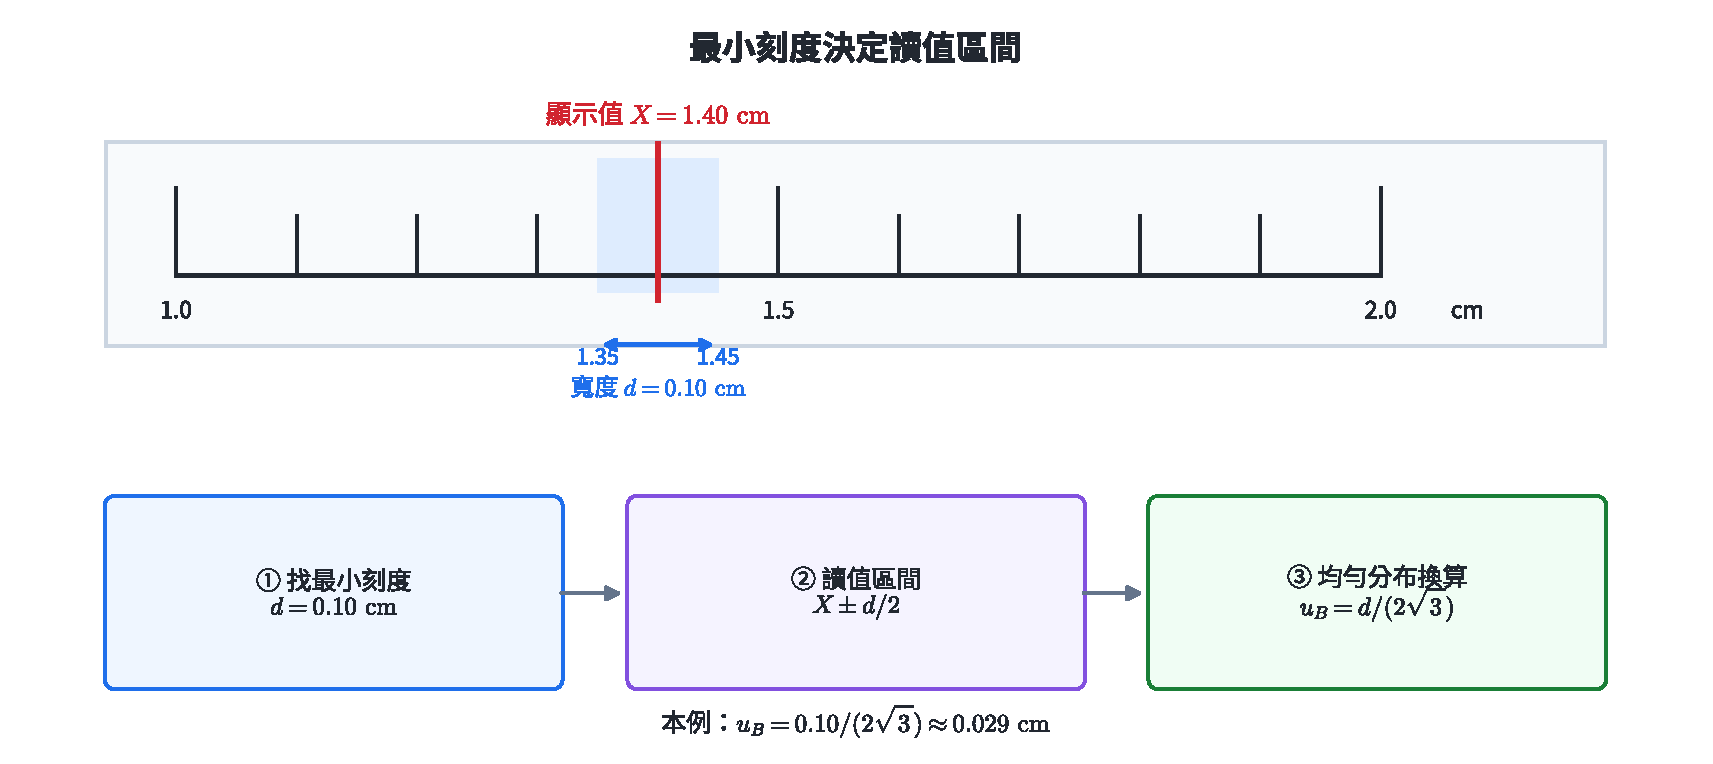
\includegraphics[width=0.96\linewidth,height=\textheight,keepaspectratio,alt={圖 2｜最小刻度 d 先建立寬度為 d 的均勻讀值區間；其半寬是 d/2，標準不確定度為 u\_B=d/(2\textbackslash sqrt3)。}]{assets/選物I-1-解析度與讀值區間.pdf}
\caption{圖 2｜最小刻度 \(d\) 先建立寬度為 \(d\) 的均勻讀值區間；其半寬是 \(d/2\)，標準不確定度為 \(u_B=d/(2\sqrt3)\)。}
\end{figure}

\begin{HandoutWorkedExample}

\subsection{完整示範｜由五次讀數合成 A 類與 B 類}\label{ux5b8cux6574ux793aux7bc4ux7531ux4e94ux6b21ux8b80ux6578ux5408ux6210-a-ux985eux8207-b-ux985e}

用最小刻度 \(d=0.10\ \mathrm{cm}\) 的尺量同一長度五次：

\[
20.1,\ 20.3,\ 20.2,\ 20.2,\ 20.2\ \mathrm{cm}.
\]

平均值為 \(\bar x=20.2\ \mathrm{cm}\)。五個偏差的平方和為

\[
(-0.1)^2+(0.1)^2+0^2+0^2+0^2=0.020\ \mathrm{cm^2},
\]

所以

\[
s=\sqrt{\frac{0.020}{4}}=0.0707\ \mathrm{cm},\qquad
u_A=\frac{0.0707}{\sqrt5}=0.0316\ \mathrm{cm}.
\]

解析度模型給出

\[
u_B=\frac{0.10}{2\sqrt3}=0.0289\ \mathrm{cm}.
\]

兩項代表不同來源，合成後

\[
u=\sqrt{0.0316^2+0.0289^2}=0.0428\ \mathrm{cm}.
\]

依本章記錄規則，\(u\) 記為 \(0.043\ \mathrm{cm}\)，平均值末位對齊，結果為

\[
\boxed{x=(20.200\pm0.043)\ \mathrm{cm}}.
\]

\end{HandoutWorkedExample}

\begin{HandoutWorkedExample}

\subsection{完整示範｜校正證書提供 B 類資訊}\label{ux5b8cux6574ux793aux7bc4ux6821ux6b63ux8b49ux66f8ux63d0ux4f9b-b-ux985eux8cc7ux8a0a}

某電壓感測器在相同條件下獨立量測 \(N=25\) 次，平均值為 \(8.420\ \mathrm V\)，樣本標準差為 \(s=0.050\ \mathrm V\)；資料沒有顯示時間漂移。校正證書另列擴展不確定度 \(U_{\mathrm{cal}}=0.040\ \mathrm V\)，涵蓋因子為 \(k=2\)。重複讀數散布與校正資訊代表不同來源。

\textbf{步驟 1──由重複測量求 A 類標準不確定度}

\[
u_A=\frac{s}{\sqrt N}
=\frac{0.050\ \mathrm V}{\sqrt{25}}
=0.010\ \mathrm V.
\]

\textbf{步驟 2──把證書數值換成 B 類標準不確定度}

證書給的是 \(U_{\mathrm{cal}}=k u_B\)，因此

\[
u_B=\frac{U_{\mathrm{cal}}}{k}
=\frac{0.040\ \mathrm V}{2}
=0.020\ \mathrm V.
\]

\textbf{步驟 3──比較來源}

\(u_B=2u_A\)，目前校正資訊的標準不確定度較大。若量測目標要求再降低總不確定度，改善校正品質或更換感測器會比只增加重複次數更直接；兩項的正式合成依下一節的 RSS 規則處理。

\end{HandoutWorkedExample}

\subsection{\texorpdfstring{重複測量的改善率是 \(1/\sqrt N\)}{重複測量的改善率是 1/\textbackslash sqrt N}}\label{ux91cdux8907ux6e2cux91cfux7684ux6539ux5584ux7387ux662f-1sqrt-n}

獨立的隨機起伏有時偏高、有時偏低。把 \(N\) 次結果取平均時，這些起伏會部分抵銷；但它們的平方貢獻相加，所以典型散布縮小為原來的 \(1/\sqrt N\)，不是 \(1/N\)。因此想把 \(u_A\) 減半，測量次數要增加到 4 倍。

\subsection{增加測量次數仍受其他不確定度限制}\label{ux589eux52a0ux6e2cux91cfux6b21ux6578ux4ecdux53d7ux5176ux4ed6ux4e0dux78baux5b9aux5ea6ux9650ux5236}

\(u_A=s/\sqrt N\) 只描述符合條件的隨機散布；增加測量次數能讓平均值更穩。儀器解析度、校準偏移與環境模型等 B 類資訊不會只靠重複次數消失。量測設計應先找出主要來源：溫度漂移主導時先控溫，解析度主導時更換儀器，隨機雜訊主導時再增加取樣與平均。

\begin{HandoutSelfCheck}

\subsection{練習}\label{ux7df4ux7fd2-2}

\begin{enumerate}
\def\labelenumi{\arabic{enumi}.}
\tightlist
\item
  某組數據的樣本標準差為 \(0.12\ \mathrm{s}\)，共測量 9 次。A 類標準不確定度是多少？
\item
  同一方法的 \(s\) 大致不變。把測量次數從 16 次增加到 64 次，\(u_A\) 變為原來幾倍？
\item
  儀器最小刻度為 \(0.20\ \mathrm{V}\)，採均勻分布模型時，求 \(u_B\)。
\item
  四次讀數完全相同，能否把完整不確定度直接寫成 0？寫出仍須評估的一類資訊。
\item
  讀數隨時間穩定上升。這組資料是否適合直接用 \(u_A=s/\sqrt N\) 描述同一固定量？
\end{enumerate}

\textbf{答案：}1. \(u_A=s/\sqrt N=0.12/3=0.04\ \mathrm{s}\)。2. \(\sqrt{16/64}=1/2\)。3. \(u_B=0.20/(2\sqrt3)=0.0577\ \mathrm{V}\)。4. 仍須評估解析度、校準資料等 B 類資訊。5. 不適合；持續漂移表示測量條件或待測量正在改變，應先找出時間趨勢並重新建立模型。

\end{HandoutSelfCheck}

\section{4. 合成與報告：把不同來源整理成一個結果}\label{ux5408ux6210ux8207ux5831ux544aux628aux4e0dux540cux4f86ux6e90ux6574ux7406ux6210ux4e00ux500bux7d50ux679c}

同一組重複測量通常同時有 A 類與 B 類資訊。本章處理最常見的情形：\(u_A\) 與 \(u_B\) 代表不同、沒有重複計入的貢獻，並可視為彼此不相關。在此前提下，依 114 課本採用的 GUM 方法，合成標準不確定度為

\[
\boxed{u=\sqrt{u_A^2+u_B^2}}.
\]

這種「先平方、相加、再開根號」稱為\textbf{平方和開根號}，英文常縮寫為 RSS（root sum square）。

每項影響只計入一次；已反映在重複讀數散布中的貢獻不再重複合成。

\begin{figure}
\centering
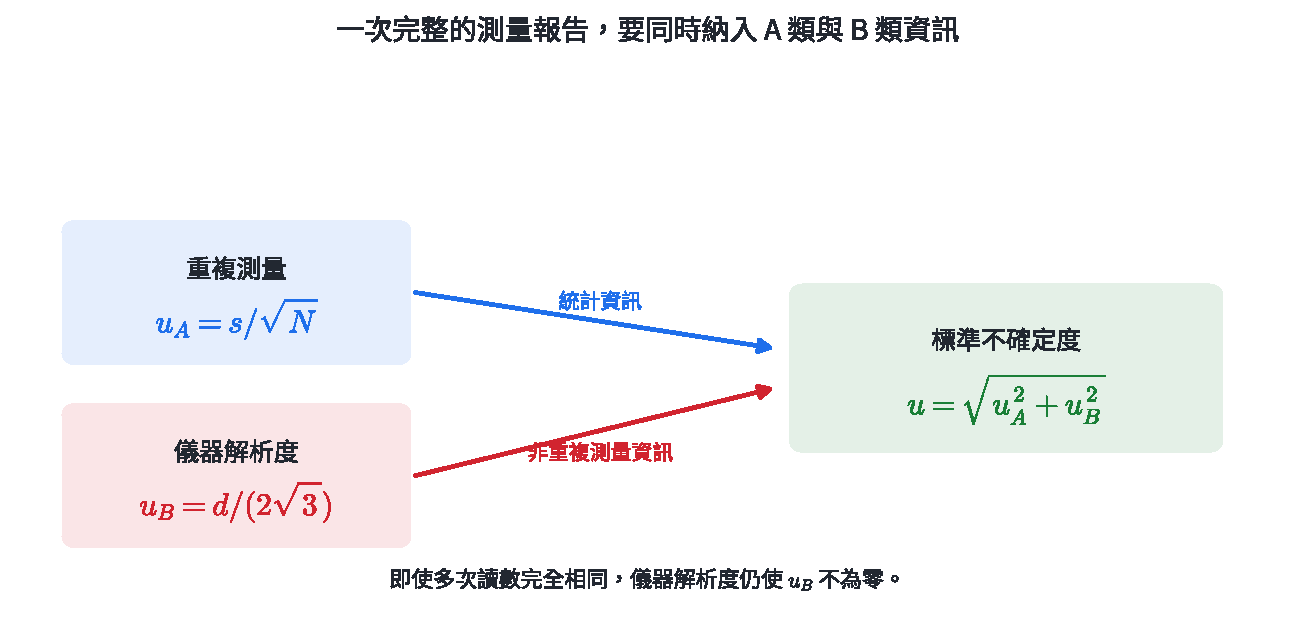
\includegraphics[width=0.96\linewidth,height=\textheight,keepaspectratio,alt={圖 3｜A 類由重複測量取得，B 類由儀器等其他資訊取得；兩者以 RSS 合成標準不確定度。}]{assets/選物I-1-標準不確定度組合.pdf}
\caption{圖 3｜A 類由重複測量取得，B 類由儀器等其他資訊取得；兩者以 RSS 合成標準不確定度。}
\end{figure}

\subsection{有效數字由不確定度決定}\label{ux6709ux6548ux6578ux5b57ux7531ux4e0dux78baux5b9aux5ea6ux6c7aux5b9a}

\textbf{有效數字}是測量值中有意義的數字。判讀時可用這三條：

\begin{enumerate}
\def\labelenumi{\arabic{enumi}.}
\tightlist
\item
  非零數字都有效；夾在非零數字之間的 0 也有效，例如 \(2.03\) 有 3 位有效數字。
\item
  小數前面只用來定位的 0 無效，小數末尾的 0 有效，例如 \(0.02030\) 有 4 位有效數字。
\item
  整數末尾的 0 容易含糊，改寫成科學記號最清楚。例如 \(2.0300\times10^5\) 明確表示 5 位有效數字。
\end{enumerate}

有效數字不是「計算機顯示幾位就抄幾位」。最後能保留到哪一位，必須由不確定度決定。

\begin{HandoutWorkedExample}

\subsection{完整示範｜從四次讀數到最後報告}\label{ux5b8cux6574ux793aux7bc4ux5f9eux56dbux6b21ux8b80ux6578ux5230ux6700ux5f8cux5831ux544a}

用最小刻度 \(d=0.01\ \mathrm{s}\) 的碼錶測某一段時間四次，得到

\[
2.00,\ 2.02,\ 2.04,\ 2.06\ \mathrm{s}.
\]

\textbf{步驟 1──最佳估計值}

\[
\bar x=\frac{2.00+2.02+2.04+2.06}{4}=2.03\ \mathrm{s}.
\]

\textbf{步驟 2──樣本標準差與 A 類不確定度}

四個偏差為 \(-0.03,-0.01,+0.01,+0.03\ \mathrm{s}\)，故

\[
s=\sqrt{\frac{0.03^2+0.01^2+0.01^2+0.03^2}{3}}
\approx0.0258\ \mathrm{s},
\]

\[
u_A=\frac{s}{\sqrt4}\approx0.0129\ \mathrm{s}.
\]

\textbf{步驟 3──B 類不確定度}

\[
u_B=\frac{0.01}{2\sqrt3}\approx0.00289\ \mathrm{s}.
\]

\textbf{步驟 4──合成}

\[
u=\sqrt{0.0129^2+0.00289^2}\approx0.01323\ \mathrm{s}.
\]

\textbf{步驟 5──依規則記錄}

本章依 114 教材採用一致的記錄慣例：不確定度最多保留 2 位有效數字；保留位置的下一位若為 1～9，一律進位，若為 0 則不進位。因此 \(0.01323\ \mathrm{s}\) 記為 \(0.014\ \mathrm{s}\)。最佳估計值以四捨五入處理，末位與不確定度末位對齊：

\[
\boxed{x=(2.030\pm0.014)\ \mathrm{s}}.
\]

\end{HandoutWorkedExample}

\begin{HandoutWorkedExample}

\subsection{完整示範｜合成後依不確定度決定位數}\label{ux5b8cux6574ux793aux7bc4ux5408ux6210ux5f8cux4f9dux4e0dux78baux5b9aux5ea6ux6c7aux5b9aux4f4dux6578}

某電流的最佳估計值為 \(X=4.3762\ \mathrm A\)。A 類與 B 類標準不確定度分別為

\[
u_A=0.0178\ \mathrm A,
\qquad
u_B=0.0115\ \mathrm A.
\]

兩項來自不同來源、沒有重複計入，且可視為彼此不相關。

\textbf{步驟 1──用 RSS 合成}

\[
u=\sqrt{u_A^2+u_B^2}
=\sqrt{(0.0178)^2+(0.0115)^2}\ \mathrm A
=0.02119\ldots\ \mathrm A.
\]

\textbf{步驟 2──修約不確定度}

不確定度最多保留 2 位有效數字，下一位非 0 時向上進位：

\[
0.02119\ldots\ \mathrm A\longrightarrow0.022\ \mathrm A.
\]

\textbf{步驟 3──對齊最佳估計值末位}

\(u\) 的末位在 \(0.001\ \mathrm A\)，因此 \(X\) 四捨五入到同一位：

\[
4.3762\ \mathrm A\longrightarrow4.376\ \mathrm A.
\]

最後報告為

\[
\boxed{I=(4.376\pm0.022)\ \mathrm A}.
\]

最佳估計值保留到 \(0.001\ \mathrm A\)，是由合成不確定度的末位決定。

\end{HandoutWorkedExample}

\subsection{114 教材的報告規則整理}\label{ux6559ux6750ux7684ux5831ux544aux898fux5247ux6574ux7406}

\begin{enumerate}
\def\labelenumi{\arabic{enumi}.}
\tightlist
\item
  中間計算多保留幾位，最後報告時再修約。
\item
  最終 \(u\) 最多保留 2 位有效數字；下一位非 0 就向上進位，下一位為 0 則不進位。
\item
  \(X\) 以一般四捨五入修約，使末位與 \(u\) 的末位對齊。
\item
  單位寫在整個括號後：\((X\pm u)\ \text{單位}\)。
\end{enumerate}

\begin{HandoutSelfCheck}

\subsection{練習}\label{ux7df4ux7fd2-3}

\begin{enumerate}
\def\labelenumi{\arabic{enumi}.}
\tightlist
\item
  若 \(u_A=0\)，完整標準不確定度應如何判定？
\item
  \(u_A=0.060\ \mathrm{g}\)、\(u_B=0.080\ \mathrm{g}\)，求合成 \(u\)。
\item
  \(X=4.3762\ \mathrm{A}\)、計算所得 \(u=0.02134\ \mathrm{A}\)。依本章規則完成報告。
\item
  為何中間步驟宜多保留幾位，最後才修約？
\end{enumerate}

\textbf{答案：}1. \(u_A=0\) 只表示重複讀數沒有顯示散布；仍須評估儀器解析度等 B 類資訊。2. \(u=\sqrt{0.060^2+0.080^2}=0.100\ \mathrm{g}\)。3. \(u\) 保留兩位有效數字並進位為 \(0.022\ \mathrm{A}\)，故 \((4.376\pm0.022)\ \mathrm{A}\)。4. 過早修約會把額外的捨入偏差帶進後續平方、開根號與比例計算。

\end{HandoutSelfCheck}

\section{5. 不確定度的傳遞：獨立貢獻仍用 RSS}\label{ux4e0dux78baux5b9aux5ea6ux7684ux50b3ux905eux7368ux7acbux8ca2ux737bux4ecdux7528-rss}

以下公式適用於 \(x\)、\(y\) 是\textbf{彼此獨立測量}，而且 \(u_x,u_y\) 都是標準不確定度的情形。若兩個量共享同一儀器偏移或由同一筆數據重複算出，它們可能相關，不能直接套本節公式。

加減關係是線性的；乘除的相對不確定度公式則適用於 \(X,Y\ne0\)，且相對不確定度不大的情形。它是本章依 114 教材採用的一階近似。

\subsection{加法與減法：合成絕對不確定度}\label{ux52a0ux6cd5ux8207ux6e1bux6cd5ux5408ux6210ux7d55ux5c0dux4e0dux78baux5b9aux5ea6}

若 \(z=x+y\) 或 \(z=x-y\)，最佳估計值分別為 \(Z=X+Y\) 或 \(Z=X-Y\)，而

\[
\boxed{u_z=\sqrt{u_x^2+u_y^2}}.
\]

加法與減法使用同一條式子，因為不確定度描述的是散布大小；平方後不保留正負號。

\begin{HandoutWorkedExample}

\subsection{加減示範}\label{ux52a0ux6e1bux793aux7bc4}

兩段獨立量得的長度為 \((12.0\pm0.3)\ \mathrm{cm}\) 與 \((8.0\pm0.4)\ \mathrm{cm}\)。總長最佳估計值為 \(20.0\ \mathrm{cm}\)，不確定度為

\[
u=\sqrt{0.3^2+0.4^2}=0.5\ \mathrm{cm}.
\]

因此總長為 \((20.0\pm0.5)\ \mathrm{cm}\)。若改求兩者之差，不確定度仍是 \(0.5\ \mathrm{cm}\)，不是 \(0.3-0.4\)。

\end{HandoutWorkedExample}

\subsection{乘法與除法：合成相對不確定度}\label{ux4e58ux6cd5ux8207ux9664ux6cd5ux5408ux6210ux76f8ux5c0dux4e0dux78baux5b9aux5ea6}

若 \(z=xy\)，則

\[
\boxed{
u_z=|XY|\sqrt{\left(\frac{u_x}{X}\right)^2+
                   \left(\frac{u_y}{Y}\right)^2}
}.
\]

若 \(z=x/y\)，則

\[
\boxed{
u_z=\left|\frac{X}{Y}\right|
\sqrt{\left(\frac{u_x}{X}\right)^2+
      \left(\frac{u_y}{Y}\right)^2}
}.
\]

兩式也可統一寫成相對形式：

\[
\boxed{
\frac{u_z}{|Z|}
=\sqrt{\left(\frac{u_x}{|X|}\right)^2+
       \left(\frac{u_y}{|Y|}\right)^2}
}.
\]

\begin{figure}
\centering
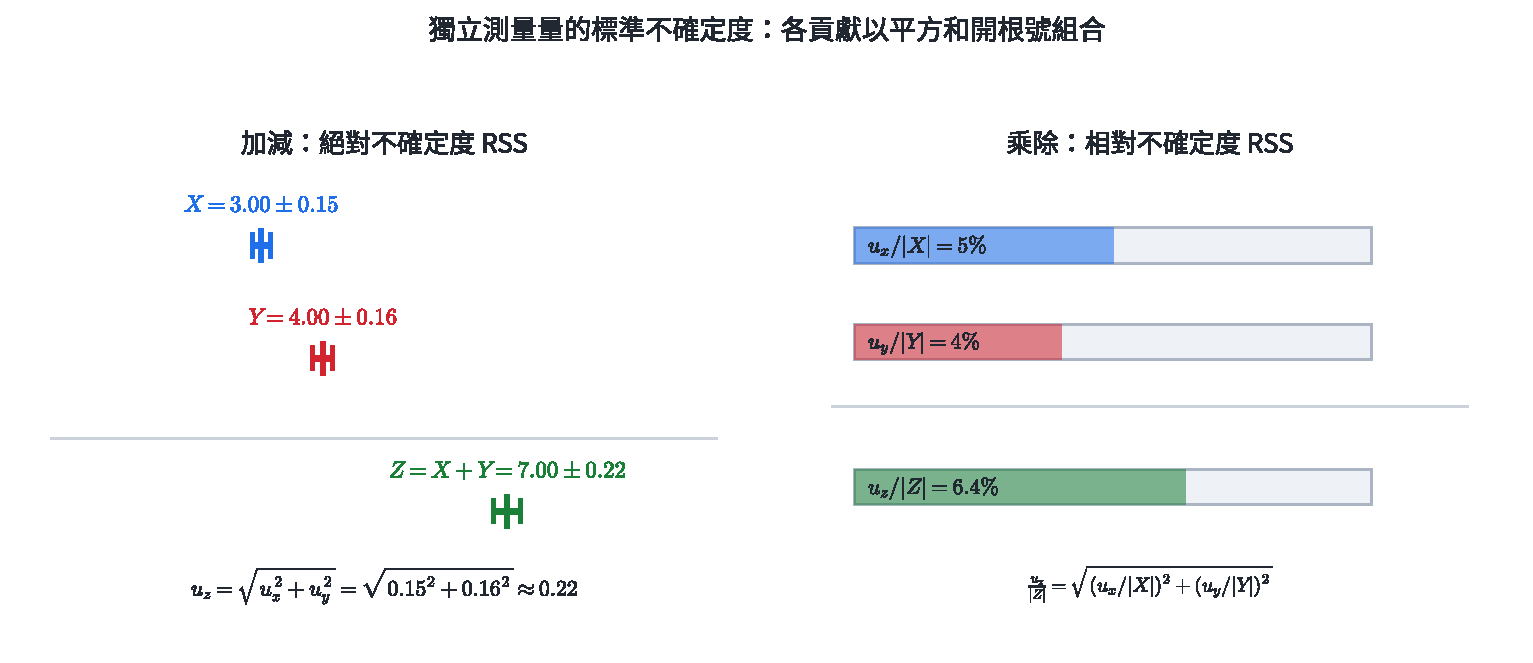
\includegraphics[width=0.96\linewidth,height=\textheight,keepaspectratio,alt={圖 4｜獨立量的加減使用絕對不確定度 RSS，乘除使用相對不確定度 RSS。}]{assets/選物I-1-不確定度傳遞.pdf}
\caption{圖 4｜獨立量的加減使用絕對不確定度 RSS，乘除使用相對不確定度 RSS。}
\end{figure}

\begin{HandoutWorkedExample}

\subsection{乘法示範｜長乘寬得到面積}\label{ux4e58ux6cd5ux793aux7bc4ux9577ux4e58ux5becux5f97ux5230ux9762ux7a4d}

獨立量得長 \(L=(12.0\pm0.1)\ \mathrm{cm}\)、寬 \(W=(8.0\pm0.2)\ \mathrm{cm}\)。面積最佳估計值為

\[
A=LW=96.0\ \mathrm{cm^2}.
\]

面積的相對不確定度為

\[
\frac{u_{\mathrm{area}}}{A}
=\sqrt{\left(\frac{0.1}{12.0}\right)^2+
       \left(\frac{0.2}{8.0}\right)^2}
\approx0.02635.
\]

所以 \(u_{\mathrm{area}}\approx96.0\times0.02635=2.53\ \mathrm{cm^2}\)。依本章報告規則，\(u_{\mathrm{area}}\) 記為 \(2.6\ \mathrm{cm^2}\)，最佳估計值末位對齊：

\[
\boxed{A=(96.0\pm2.6)\ \mathrm{cm^2}}.
\]

\end{HandoutWorkedExample}

\subsection{獨立標準不確定度以 RSS 合成}\label{ux7368ux7acbux6a19ux6e96ux4e0dux78baux5b9aux5ea6ux4ee5-rss-ux5408ux6210}

若各來源獨立，有的偏高、有的偏低，不會每次都同時朝同一方向偏。標準不確定度對應散布；獨立散布的\textbf{平方}會相加，因此最後取平方和的平方根。直接相加屬於另一種線性合成慣例；只有把輸入另解讀為有界的最大容許偏差時，才可賦予「最壞情況」意義。它不能和本章的標準不確定度公式混用。

\subsection{感測器融合需要量化每筆資料的可信程度}\label{ux611fux6e2cux5668ux878dux5408ux9700ux8981ux91cfux5316ux6bcfux7b46ux8cc7ux6599ux7684ux53efux4fe1ux7a0bux5ea6}

機器人、無人機與手機常同時取得相機、慣性感測器與衛星定位資料。各來源的不確定度可用來配置權重，避免高雜訊資料過度拉動結果。不同感測器也可能共享同一時鐘、溫度或校準偏移而彼此相關；相關貢獻不適用獨立來源的 RSS。這是公式要求「彼此獨立／不相關」的實務原因。

\begin{HandoutSelfCheck}

\subsection{練習}\label{ux7df4ux7fd2-4}

\begin{enumerate}
\def\labelenumi{\arabic{enumi}.}
\tightlist
\item
  兩個獨立量的標準不確定度都是 \(0.20\ \mathrm{m}\)。它們相減所得結果的標準不確定度是 \(0\)、\(0.20\)、\(0.28\) 還是 \(0.40\ \mathrm{m}\)？
\item
  \(x=(5.0\pm0.1)\ \mathrm{cm}\)、\(y=(2.0\pm0.2)\ \mathrm{cm}\)，求 \(x+y\) 與 \(x-y\) 的標準不確定度。
\item
  \(L=(10.0\pm0.2)\ \mathrm{cm}\)，只用同一次 \(L\) 算正方形面積 \(L^2\)。這個問題能否把兩個 \(L\) 當成彼此獨立後直接套雙變量 RSS？
\item
  \(m=(2.00\pm0.02)\ \mathrm{kg}\)、\(V=(0.500\pm0.010)\ \mathrm{m^3}\)，以 \(\rho=m/V\) 求相對標準不確定度。
\item
  乘除傳遞式要求相對不確定度不大。若輸入接近 0，為何要重新檢查模型？
\end{enumerate}

\textbf{答案：}1. \(\sqrt{0.20^2+0.20^2}\approx0.28\ \mathrm{m}\)。2. 兩者皆為 \(\sqrt{0.1^2+0.2^2}=0.224\ \mathrm{cm}\)。3. 不能；兩個因子來自同一筆 \(L\)，彼此完全相關，本節雙變量獨立公式不適用。4. \(u_\rho/\rho=\sqrt{(0.02/2.00)^2+(0.010/0.500)^2}=0.0224\)，約 \(2.24\%\)。5. 除以接近 0 的估計值會使相對量失去穩定意義，一階近似也可能失效。

\end{HandoutSelfCheck}

\section{6. 因次分析：以因次檢查公式可行性}\label{ux56e0ux6b21ux5206ux6790ux4ee5ux56e0ux6b21ux6aa2ux67e5ux516cux5f0fux53efux884cux6027}

\textbf{單位（unit）}是選來表達數值的標準，例如速度可用 \(\mathrm{m/s}\) 或 \(\mathrm{km/h}\)；\textbf{因次（dimension）}描述物理量由哪些基本物理量組成，不隨選用單位而改變。

SI 有七個基本物理量：時間、長度、質量、電流、熱力學溫度、物質量與光強度。力學最常用其中三個因次：

{\def\LTcaptype{none} % do not increment counter
\begin{longtable}[]{@{}lll@{}}
\toprule\noalign{}
基本量 & SI 單位 & 因次符號 \\
\midrule\noalign{}
\endhead
\bottomrule\noalign{}
\endlastfoot
長度 & 公尺 \(\mathrm{m}\) & \(L\) \\
質量 & 公斤 \(\mathrm{kg}\) & \(M\) \\
時間 & 秒 \(\mathrm{s}\) & \(T\) \\
\end{longtable}
}

常見例子：

\[
[v]=LT^{-1},\qquad
[a]=LT^{-2},\qquad
[F]=MLT^{-2},\qquad
[E]=ML^2T^{-2}.
\]

物理等式兩邊的因次必須相同，等號兩側相加的每一項也必須有相同因次。例如

\[
x=v_0t+\frac12at^2
\]

中，\([v_0t]=(LT^{-1})T=L\)，\([at^2]=(LT^{-2})T^2=L\)，兩項都能與位移 \(x\) 相加。

\begin{figure}
\centering
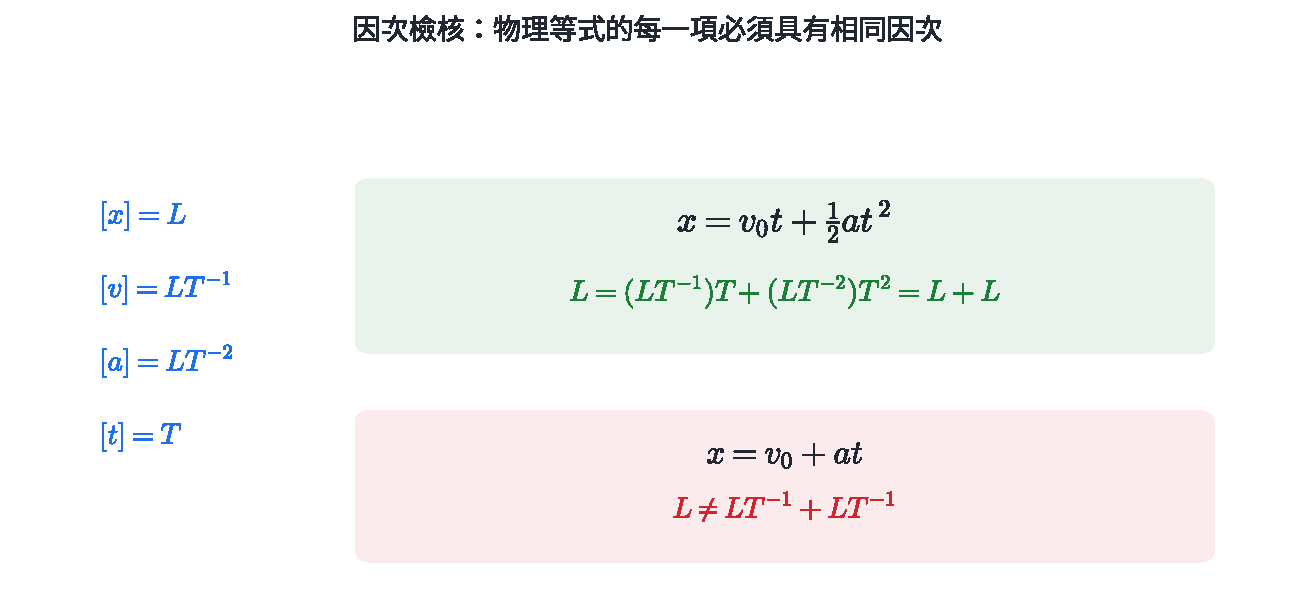
\includegraphics[width=0.96\linewidth,height=\textheight,keepaspectratio,alt={圖 5｜因次檢核先確認可相加的每一項與等號兩邊具有相同因次；因次不合的式子一定錯。}]{assets/選物I-1-因次檢核.pdf}
\caption{圖 5｜因次檢核先確認可相加的每一項與等號兩邊具有相同因次；因次不合的式子一定錯。}
\end{figure}

\begin{HandoutWorkedExample}

\subsection{完整示範｜用因次找出公式形式}\label{ux5b8cux6574ux793aux7bc4ux7528ux56e0ux6b21ux627eux51faux516cux5f0fux5f62ux5f0f}

假設向心加速度大小 \(a\) 與速率 \(v\)、半徑 \(r\) 的關係可寫成

\[
a=kv^p r^q,
\]

其中 \(k\) 無因次。兩側因次為

\[
LT^{-2}=(LT^{-1})^pL^q=L^{p+q}T^{-p}.
\]

比較時間次方得 \(-p=-2\)，所以 \(p=2\)；比較長度次方得 \(p+q=1\)，所以 \(q=-1\)。因此

\[
a=k\frac{v^2}{r}.
\]

因次分析找得到 \(v^2/r\) 的形式，卻無法決定無因次常數 \(k\) 的數值。

\end{HandoutWorkedExample}

\begin{HandoutWorkedExample}

\subsection{完整示範｜檢查等加速度關係的每一項}\label{ux5b8cux6574ux793aux7bc4ux6aa2ux67e5ux7b49ux52a0ux901fux5ea6ux95dcux4fc2ux7684ux6bcfux4e00ux9805}

候選式

\[
v^2=v_0^2+2a\Delta x
\]

左側因次為

\[
[v^2]=(LT^{-1})^2=L^2T^{-2}.
\]

右側第一項 \([v_0^2]=L^2T^{-2}\)；第二項

\[
[2a\Delta x]=1\cdot(LT^{-2})L=L^2T^{-2}.
\]

三項因次一致，因此式子通過因次檢核。係數 2 沒有因次，因次分析無法判定它是 2、1 或其他純數；係數須由運動定義與推導決定。

若候選式誤寫成 \(v=v_0+2a\Delta x\)，最後一項因次為 \(L^2T^{-2}\)，無法與速度相加，立即可排除。

\end{HandoutWorkedExample}

\subsection{常見錯誤｜因次相同就一定是同一個物理量}\label{ux5e38ux898bux932fux8aa4ux56e0ux6b21ux76f8ux540cux5c31ux4e00ux5b9aux662fux540cux4e00ux500bux7269ux7406ux91cf}

功與動能都有 \(ML^2T^{-2}\)，卻不是同一概念。因次相同只是公式可能成立的\textbf{必要條件}，不是充分證明；正負號、方向、無因次常數與物理條件仍須另外判斷。

\subsection{單位與因次檢查是工程安全機制}\label{ux55aeux4f4dux8207ux56e0ux6b21ux6aa2ux67e5ux662fux5de5ux7a0bux5b89ux5168ux6a5fux5236}

感測器可能輸出公尺、公里、秒、毫秒或角度；混用會讓速度、加速度或軌道估計差上數個數量級。因次檢核能在執行昂貴模擬或控制命令之前，排除物理量種類不相容的錯誤。公尺與公里的因次同為 \(L\)，因此倍率錯誤仍須靠明確記錄單位、轉換測試與已知情境的量級驗證發現。

\begin{HandoutSelfCheck}

\subsection{練習}\label{ux7df4ux7fd2-5}

\begin{enumerate}
\def\labelenumi{\arabic{enumi}.}
\tightlist
\item
  公式 \(v=v_0+at^2\) 能否成立？
\item
  動量 \(p=mv\) 的因次為何？
\item
  功率定義為能量除以時間。寫出功率的因次。
\item
  式子 \(x=A\sin(\omega t)\) 中，\(A\) 與 \(\omega\) 各應具有什麼因次？
\item
  兩個公式因次完全相同，是否足以證明它們描述同一物理定律？
\end{enumerate}

\textbf{答案：}1. 不能；\([at^2]=L\)，無法與速度相加。2. \([p]=MLT^{-1}\)。3. \([P]=ML^2T^{-3}\)。4. 正弦的自變量須無因次，所以 \([\omega]=T^{-1}\)；\([A]=L\)。5. 不足；因次一致只是必要條件，係數、方向、初始條件與物理機制仍須核對。

\end{HandoutSelfCheck}

\section{7. 一頁核心整理}\label{ux4e00ux9801ux6838ux5fc3ux6574ux7406}

\subsection{從原始數據到測量結果}\label{ux5f9eux539fux59cbux6578ux64daux5230ux6e2cux91cfux7d50ux679c}

\[
\bar x=\frac1N\sum x_i,
\qquad
s=\sqrt{\frac{1}{N-1}\sum(x_i-\bar x)^2},
\]

\[
u_A=\frac{s}{\sqrt N},
\qquad
u_B=\frac{d}{2\sqrt3},
\qquad
u=\sqrt{u_A^2+u_B^2}.
\]

\begin{itemize}
\tightlist
\item
  A 類與 B 類是取得不確定度的兩種方法，不是隨機／系統的另一個名稱，也沒有高低之分。
\item
  合成前先確認各項代表不同、未重複計入且可視為不相關的貢獻。
\item
  依 114 教材記錄規則，\(u\) 最多保留 2 位有效數字，依「下一位非 0 就進位」處理；\(X\) 末位與 \(u\) 對齊。
\item
  測量結果寫成 \((X\pm u)\ \text{單位}\)。
\end{itemize}

\subsection{獨立測量值的傳遞}\label{ux7368ux7acbux6e2cux91cfux503cux7684ux50b3ux905e}

\begin{itemize}
\tightlist
\item
  加減：\(u_z=\sqrt{u_x^2+u_y^2}\)。
\item
  乘除：在 \(X,Y\ne0\)、相對不確定度不大時，以一階近似
  \(u_z/|Z|=\sqrt{(u_x/|X|)^2+(u_y/|Y|)^2}\)。
\item
  先確認輸入量彼此獨立；相關量不直接套用本章公式。
\end{itemize}

\subsection{因次分析}\label{ux56e0ux6b21ux5206ux6790}

\begin{itemize}
\tightlist
\item
  等式兩邊與可相加的各項必須有相同因次。
\item
  因次正確只建立「可能成立」的必要條件；物理推理與實驗提供進一步判定。
\end{itemize}

\section{8. 代表題：綜合練習}\label{ux4ee3ux8868ux984cux7d9cux5408ux7df4ux7fd2}

\subsection{題目 1｜不確定度來源}\label{ux984cux76ee-1ux4e0dux78baux5b9aux5ea6ux4f86ux6e90}

用光電計時器測小球落下時間時，出現以下情況：甲，小球釋放位置每次略有不同；乙，計時器解析度有限；丙，實驗桌受到走動造成的振動；丁，操作者判斷小球是否完全靜止。請分別判斷主要來源。

\subsection{題目 2｜C2 可略：準確與精密}\label{ux984cux76ee-2c2-ux53efux7565ux6e96ux78baux8207ux7cbeux5bc6}

可信參考值為 \(50.0\ \mathrm{g}\)。甲組四次皆為 \(52.0\ \mathrm{g}\)；乙組為 \(49.7,50.2,50.0,50.1\ \mathrm{g}\)。哪組較精密？哪組較接近參考值？多測甲組能否自動消除其共同偏移？

\subsection{題目 3｜A 類評估}\label{ux984cux76ee-3a-ux985eux8a55ux4f30}

某長度測量四次為 \(5.0,5.2,4.8,5.0\ \mathrm{cm}\)。求平均值、樣本標準差 \(s\) 與 A 類標準不確定度 \(u_A\)。

\subsection{題目 4｜B 類、合成與報告}\label{ux984cux76ee-4b-ux985eux5408ux6210ux8207ux5831ux544a}

某測量的最佳估計值為 \(12.345\ \mathrm{cm}\)，已知 \(u_A=0.040\ \mathrm{cm}\)，儀器最小刻度 \(d=0.10\ \mathrm{cm}\)。求 \(u_B\)、合成標準不確定度 \(u\)，並依本章規則報告結果。

\subsection{題目 5｜加減的傳遞}\label{ux984cux76ee-5ux52a0ux6e1bux7684ux50b3ux905e}

獨立量得 \(x=(18.0\pm0.3)\ \mathrm{cm}\)、\(y=(7.0\pm0.4)\ \mathrm{cm}\)。求 \(z=x-y\) 的最佳估計值與標準不確定度。

\subsection{題目 6｜除法的傳遞}\label{ux984cux76ee-6ux9664ux6cd5ux7684ux50b3ux905e}

獨立量得路程 \(s=(100.0\pm0.5)\ \mathrm{m}\)、時間 \(t=(20.0\pm0.2)\ \mathrm{s}\)。以 \(v=s/t\) 求速率及其標準不確定度，並完成報告。

\subsection{題目 7｜記錄位數}\label{ux984cux76ee-7ux8a18ux9304ux4f4dux6578}

計算得到最佳估計值 \(X=7.24681\ \mathrm{m}\)、標準不確定度 \(u=0.05304\ \mathrm{m}\)。依本章規則應如何記錄？

\subsection{題目 8｜因次分析}\label{ux984cux76ee-8ux56e0ux6b21ux5206ux6790}

假設單擺週期 \(P\) 只與擺長 \(\ell\)、重力加速度 \(g\) 有關，可寫成 \(P=k\ell^a g^b\)，其中 \(k\) 無因次。用因次分析求 \(a,b\)。

\subsection{題目 9｜樣本標準差與平均值不確定度}\label{ux984cux76ee-9ux6a23ux672cux6a19ux6e96ux5deeux8207ux5e73ux5747ux503cux4e0dux78baux5b9aux5ea6}

某電壓的 9 次讀值具有樣本標準差 \(s=0.18\ \mathrm{V}\)。若測量條件不變，分別求 9 次平均與 36 次平均的 A 類標準不確定度，並比較改善倍率。

\subsection{題目 10｜解析度與合成}\label{ux984cux76ee-10ux89e3ux6790ux5ea6ux8207ux5408ux6210}

某數位儀表最小顯示位為 \(d=0.020\ \mathrm{A}\)，重複測量得到 \(u_A=0.010\ \mathrm{A}\)。採本章均勻分布模型，求 \(u_B\) 與合成標準不確定度。

\subsection{題目 11｜獨立量相加}\label{ux984cux76ee-11ux7368ux7acbux91cfux76f8ux52a0}

兩段獨立測得的位移為 \((3.20\pm0.05)\ \mathrm{m}\) 與 \((-1.10\pm0.08)\ \mathrm{m}\)。求總位移的最佳估計值與標準不確定度。

\subsection{題目 12｜面積的傳遞}\label{ux984cux76ee-12ux9762ux7a4dux7684ux50b3ux905e}

長方形兩邊獨立量得 \(L=(15.0\pm0.2)\ \mathrm{cm}\)、\(W=(4.00\pm0.05)\ \mathrm{cm}\)。求面積與其標準不確定度，依本章規則報告。

\subsection{題目 13｜因次排除候選式}\label{ux984cux76ee-13ux56e0ux6b21ux6392ux9664ux5019ux9078ux5f0f}

下列哪一個量具有能量因次 \(ML^2T^{-2}\)？

\begin{enumerate}
\def\labelenumi{\arabic{enumi}.}
\tightlist
\item
  \(mv\)
\item
  \(ma\)
\item
  \(mv^2\)
\item
  \(m/v\)
\end{enumerate}

逐一寫出因次後判定。

\subsection{題目 14｜跨節整合：由時間資料得到速率}\label{ux984cux76ee-14ux8de8ux7bc0ux6574ux5408ux7531ux6642ux9593ux8cc7ux6599ux5f97ux5230ux901fux7387}

小車通過長度為 \(s=(1.200\pm0.006)\ \mathrm{m}\) 的測量區，時間為 \(t=(0.800\pm0.010)\ \mathrm{s}\)，兩量可視為獨立。以 \(v=s/t\) 求速率與標準不確定度，並以因次檢查結果的單位。

\subsection{題目 15｜跨節整合：重複讀數、解析度與報告}\label{ux984cux76ee-15ux8de8ux7bc0ux6574ux5408ux91cdux8907ux8b80ux6578ux89e3ux6790ux5ea6ux8207ux5831ux544a}

用最小刻度 \(d=0.20\ \mathrm{g}\) 的電子秤量同一物體四次，得到

\[
50.0,\ 50.2,\ 49.8,\ 50.0\ \mathrm{g}.
\]

求 \(\bar x,s,u_A,u_B,u\)，並依本章規則報告。A、B 兩項視為不相關且未重複計入。

\subsection{題目 16｜跨節整合：設計能回答問題的量測}\label{ux984cux76ee-16ux8de8ux7bc0ux6574ux5408ux8a2dux8a08ux80fdux56deux7b54ux554fux984cux7684ux91cfux6e2c}

某同學想判斷金屬棒受熱後是否真的伸長約 \(0.10\ \mathrm{mm}\)。現有尺的最小刻度為 \(1\ \mathrm{mm}\)，且室溫在測量期間持續改變。請依「被測物、儀器、環境、測量者」四類來源，提出至少三項具體改進；再說明只把測量次數增加到 100 次，為何仍未必能回答問題。

\section{9. 代表題詳解}\label{ux4ee3ux8868ux984cux8a73ux89e3}

\subsection{第 1 題}\label{ux7b2c-1-ux984c}

\begin{itemize}
\tightlist
\item
  甲：被測物／待測條件；起始位置改變，實際待測過程也改變。
\item
  乙：儀器；解析度是儀器特性。
\item
  丙：環境；外界振動影響裝置。
\item
  丁：測量者；判讀標準與操作由人引入。
\end{itemize}

一項實驗常同時具有四類來源；分類用來辨認各項貢獻並改進方法。

\subsection{第 2 題}\label{ux7b2c-2-ux984c}

甲組四次完全相同，因此較精密；但四次都比參考值高 \(2.0\ \mathrm{g}\)。乙組略有散布，平均為

\[
\frac{49.7+50.2+50.0+50.1}{4}=50.0\ \mathrm{g},
\]

較接近參考值。甲組的共同偏移需要校準或改變方法，多測幾次不會自動消除。

\subsection{第 3 題}\label{ux7b2c-3-ux984c}

平均值為

\[
\bar x=\frac{5.0+5.2+4.8+5.0}{4}=5.0\ \mathrm{cm}.
\]

四個偏差為 \(0,+0.2,-0.2,0\ \mathrm{cm}\)，故

\[
s=\sqrt{\frac{0^2+0.2^2+(-0.2)^2+0^2}{4-1}}
=\sqrt{\frac{0.08}{3}}
\approx0.163\ \mathrm{cm}.
\]

\[
u_A=\frac{s}{\sqrt4}\approx0.0816\ \mathrm{cm}.
\]

本題只問 A 類評估。若另有\textbf{未重複計入且可視為不相關}的 B 類貢獻，完整報告時才與 \(u_A\) 合成；同一影響若已反映在讀數散布中，不可再加入一次。

\subsection{第 4 題}\label{ux7b2c-4-ux984c}

由儀器解析度得到

\[
u_B=\frac{0.10}{2\sqrt3}\approx0.0289\ \mathrm{cm}.
\]

合成標準不確定度為

\[
u=\sqrt{0.040^2+0.0289^2}
\approx0.0493\ \mathrm{cm}.
\]

最多保留兩位有效數字，\(0.0493\) 保留到 \(0.049\) 時，下一位為 3，依規則向上進位成 \(0.050\ \mathrm{cm}\)。\(X\) 末位已與之對齊，因此

\[
\boxed{x=(12.345\pm0.050)\ \mathrm{cm}}.
\]

末尾的 0 必須保留，因為它表示不確定度記到 \(0.001\ \mathrm{cm}\)。

\subsection{第 5 題}\label{ux7b2c-5-ux984c}

最佳估計值為

\[
Z=18.0-7.0=11.0\ \mathrm{cm}.
\]

兩者獨立，故

\[
u_z=\sqrt{0.3^2+0.4^2}=0.5\ \mathrm{cm}.
\]

所以

\[
\boxed{z=(11.0\pm0.5)\ \mathrm{cm}}.
\]

\subsection{第 6 題}\label{ux7b2c-6-ux984c}

最佳估計值為

\[
V=\frac{100.0}{20.0}=5.00\ \mathrm{m/s}.
\]

相對標準不確定度為

\[
\frac{u_v}{V}
=\sqrt{\left(\frac{0.5}{100.0}\right)^2+
       \left(\frac{0.2}{20.0}\right)^2}
=\sqrt{0.005^2+0.010^2}
\approx0.01118.
\]

因此

\[
u_v=5.00\times0.01118\approx0.0559\ \mathrm{m/s}.
\]

依規則記為 \(0.056\ \mathrm{m/s}\)，最佳估計值末位對齊：

\[
\boxed{v=(5.000\pm0.056)\ \mathrm{m/s}}.
\]

\subsection{第 7 題}\label{ux7b2c-7-ux984c}

\(u=0.05304\ \mathrm{m}\) 最多保留兩位有效數字。保留 \(0.053\) 時，下一位是 0，故不進位，記為 \(0.053\ \mathrm{m}\)。最佳估計值四捨五入到同一末位：

\[
\boxed{x=(7.247\pm0.053)\ \mathrm{m}}.
\]

\subsection{第 8 題}\label{ux7b2c-8-ux984c}

左側 \([P]=T\)。右側為

\[
[\ell^a g^b]=L^a(LT^{-2})^b=L^{a+b}T^{-2b}.
\]

比較時間次方：\(-2b=1\)，所以 \(b=-\tfrac12\)。比較長度次方：\(a+b=0\)，所以 \(a=\tfrac12\)。因此

\[
P=k\ell^{1/2}g^{-1/2}=k\sqrt{\frac{\ell}{g}}.
\]

因次分析無法求出無因次常數 \(k\)；單擺小角度模型中的常數須由更完整理論或實驗決定。

\subsection{第 9 題}\label{ux7b2c-9-ux984c}

9 次平均：

\[
u_{A,9}=\frac{0.18}{\sqrt9}=0.060\ \mathrm{V}.
\]

36 次平均：

\[
u_{A,36}=\frac{0.18}{\sqrt{36}}=0.030\ \mathrm{V}.
\]

次數增為 4 倍，\(u_A\) 變為 \(1/2\)。這個比較假設單次讀值散布 \(s\) 與測量條件大致不變。

\subsection{第 10 題}\label{ux7b2c-10-ux984c}

\[
u_B=\frac{0.020}{2\sqrt3}=0.00577\ \mathrm{A}.
\]

\[
u=\sqrt{0.010^2+0.00577^2}=0.01155\ \mathrm{A}.
\]

若要作最後報告，依本章規則可把不確定度記為 \(0.012\ \mathrm{A}\)，再把最佳估計值的末位對齊到 \(0.001\ \mathrm{A}\)。

\subsection{第 11 題}\label{ux7b2c-11-ux984c}

最佳估計值保留方向：

\[
Z=3.20+(-1.10)=2.10\ \mathrm{m}.
\]

獨立量相加時，絕對標準不確定度以 RSS 合成：

\[
u_z=\sqrt{0.05^2+0.08^2}=0.0943\ \mathrm{m}.
\]

依規則進位為 \(0.095\ \mathrm{m}\)，所以

\[
\boxed{z=(2.100\pm0.095)\ \mathrm{m}}.
\]

\subsection{第 12 題}\label{ux7b2c-12-ux984c}

\[
A=LW=(15.0)(4.00)=60.0\ \mathrm{cm^2}.
\]

\[
\frac{u_A}{A}
=\sqrt{\left(\frac{0.2}{15.0}\right)^2+
       \left(\frac{0.05}{4.00}\right)^2}
=0.01828.
\]

\[
u_A=(60.0)(0.01828)=1.097\ \mathrm{cm^2}.
\]

依規則將不確定度進位為 \(1.1\ \mathrm{cm^2}\)，最佳估計值末位對齊：

\[
\boxed{A=(60.0\pm1.1)\ \mathrm{cm^2}}.
\]

\subsection{第 13 題}\label{ux7b2c-13-ux984c}

\[
[mv]=MLT^{-1},\qquad
[ma]=MLT^{-2},
\]

\[
[mv^2]=M(LT^{-1})^2=ML^2T^{-2},\qquad
[m/v]=ML^{-1}T.
\]

因此第 3 項具有能量因次。因次相同仍只表示它可能與能量建立關係；完整物理量還需係數與定義。

\subsection{第 14 題}\label{ux7b2c-14-ux984c}

最佳估計值：

\[
V=\frac{1.200}{0.800}=1.500\ \mathrm{m/s}.
\]

相對標準不確定度：

\[
\frac{u_v}{V}
=\sqrt{\left(\frac{0.006}{1.200}\right)^2+
       \left(\frac{0.010}{0.800}\right)^2}
=0.01346.
\]

\[
u_v=(1.500)(0.01346)=0.0202\ \mathrm{m/s}.
\]

依規則記為 \(0.021\ \mathrm{m/s}\)，所以

\[
\boxed{v=(1.500\pm0.021)\ \mathrm{m/s}}.
\]

因次為 \([s/t]=LT^{-1}\)，與速度一致。

\subsection{第 15 題}\label{ux7b2c-15-ux984c}

平均值為 \(\bar x=50.0\ \mathrm{g}\)。偏差平方和為

\[
0^2+0.2^2+(-0.2)^2+0^2=0.08\ \mathrm{g^2}.
\]

\[
s=\sqrt{\frac{0.08}{3}}=0.1633\ \mathrm{g},\qquad
u_A=\frac{0.1633}{2}=0.08165\ \mathrm{g}.
\]

\[
u_B=\frac{0.20}{2\sqrt3}=0.05774\ \mathrm{g},
\]

\[
u=\sqrt{0.08165^2+0.05774^2}=0.1000\ \mathrm{g}.
\]

不確定度記為 \(0.10\ \mathrm{g}\)，最佳估計值末位對齊：

\[
\boxed{m=(50.00\pm0.10)\ \mathrm{g}}.
\]

\subsection{第 16 題}\label{ux7b2c-16-ux984c}

可行改進包括：

\begin{enumerate}
\def\labelenumi{\arabic{enumi}.}
\tightlist
\item
  \textbf{被測物：}固定量測位置與支撐方式，並讓金屬棒每次達到指定溫度後再讀值。
\item
  \textbf{儀器：}改用解析度明顯小於 \(0.10\ \mathrm{mm}\) 的位移感測器或螺旋測微器，並先校準零點。
\item
  \textbf{環境：}隔離氣流與振動，記錄並穩定室溫，避免支架本身熱脹冷縮混入結果。
\item
  \textbf{測量者：}固定觀測方向與讀值時刻，使用治具降低每次放置差異。
\end{enumerate}

原尺的 \(1\ \mathrm{mm}\) 刻度比預期伸長 \(0.10\ \mathrm{mm}\) 粗 10 倍，解析度造成的 B 類限制不會靠增加次數消失；持續變動的室溫也會讓待測條件改變。先改善解析度與控制條件，重複測量才有機會降低剩餘的隨機散布。


\end{document}
